\section{ Appendix : TMVA}
\label{appendix:tmva}

\begin{figure}[!htb]\centering
\includegraphics[width=0.9\textwidth]{Fig/TMVA/thad_vs_QCD/variables_id_c1.eps}
\includegraphics[width=0.9\textwidth,trim={0 5cm 0 0},clip]{Fig/TMVA/thad_vs_QCD/variables_id_c2.eps}
\caption{Input variables for top Vs QCD tagger.}
\label{fig:TMVA_inputs_t}
\end{figure}

\begin{figure}[!htb]\centering
\includegraphics[width=0.9\textwidth]{Fig/TMVA/Whad_vs_QCD/variables_id_c1.eps}
\includegraphics[width=0.9\textwidth]{Fig/TMVA/Whad_vs_QCD/variables_id_c2.eps}
\includegraphics[width=0.9\textwidth,trim={0 5cm 0 0},clip]{Fig/TMVA/Whad_vs_QCD/variables_id_c3.eps}
\caption{Input variables for W Vs QCD tagger.}
\label{fig:TMVA_inputs_w}
\end{figure}

\begin{figure}[!htb]\centering
\includegraphics[width=0.495\textwidth]{Fig/TMVA/thad_vs_QCD/CorrelationMatrixS.eps}
\includegraphics[width=0.495\textwidth]{Fig/TMVA/thad_vs_QCD/CorrelationMatrixB.eps}
\includegraphics[width=0.495\textwidth]{Fig/TMVA/Whad_vs_QCD/CorrelationMatrixS.eps}
\includegraphics[width=0.495\textwidth]{Fig/TMVA/Whad_vs_QCD/CorrelationMatrixB.eps}
\caption{Correlation matrices for Signal (left) and Background (right) for top Vs QCD tagger (top) and W Vs QCD tagger (bottom).}
\label{fig:TMVA_corr_matrix}
\end{figure}

\begin{figure}[!htb]\centering
\includegraphics[width=0.495\textwidth]{Fig/TMVA/thad_vs_QCD/overtrain_BDT_thad_vs_QCD.eps}
\includegraphics[width=0.495\textwidth]{Fig/TMVA/Whad_vs_QCD/overtrain_BDT_Whad_vs_QCD.eps}
\caption{BDT scores for Signal (red) and Background (blue) for top Vs QCD tagger (left) and W Vs QCD tagger (right).}
\label{fig:TMVA_BDTscore}
\end{figure}

\begin{figure}[!htb]\centering
\includegraphics[width=0.495\textwidth]{Fig/TMVA/thad_vs_QCD/rejBvsS.eps}
\includegraphics[width=0.495\textwidth]{Fig/TMVA/Whad_vs_QCD/rejBvsS.eps}
\caption{Top ROC curves show background rejection Vs Signal efficiency for top Vs QCD tagger (left) and W Vs QCD tagger (right).}
\label{fig:TMVA_ROC}
\end{figure}

\begin{figure}[!htb]\centering
\includegraphics[width=0.495\textwidth]{Fig/TMVA/Jet1_thad_vs_QCD_tagger.eps}
\includegraphics[width=0.495\textwidth]{Fig/TMVA/Jet2_thad_vs_QCD_tagger.eps}
\includegraphics[width=0.495\textwidth]{Fig/TMVA/Jet1_Whad_vs_QCD_tagger.eps}
\includegraphics[width=0.495\textwidth]{Fig/TMVA/Jet2_Whad_vs_QCD_tagger.eps}
\caption{Signal BDT score shapes comparison for masses from 10 to 35 $\TeV$ (and ratio to 20 $\TeV$ mass) for leading jet (left) and second leading jet $\pt$ (right) for top Vs QCD tagger (top) and W Vs QCD tagger (bottom).}
\label{fig:BDT_signal_shape_comparison}
\end{figure}

\clearpage
\newpage

%%%%%%%%%%%%%%%%%%%%%%%%%%%%%%%%%%%%%%%%%%%%%%%%%%%%%
%%%%%%%%%%%%%%%%%%%%%%%%%%%%%%%%%%%%%%%%%%%%%%%%%%%%%
\section{Appendix : \zptt\ 100 TeV}
\label{appendix:zptt100}

% useless
%\begin{figure}[!htb]\centering
%\includegraphics[width=0.8\textwidth]{Fig/Zptt/rapiditySeparation_sel0_before_cut_nostack_log.eps}
%\caption{Rapidity separation at preselection level before cut on this variable in \zptt\ analysis. The generated mass of the signal sample is 10 $\TeV$.}
%\label{fig:Zptt_sel0_rapidity}
%\end{figure}

\begin{figure}[!htb]\centering
\includegraphics[width=0.32\textwidth]{Fig/Zptt/Jet1_trk02_SD_Cor_m_sel0_nostack_log.eps}
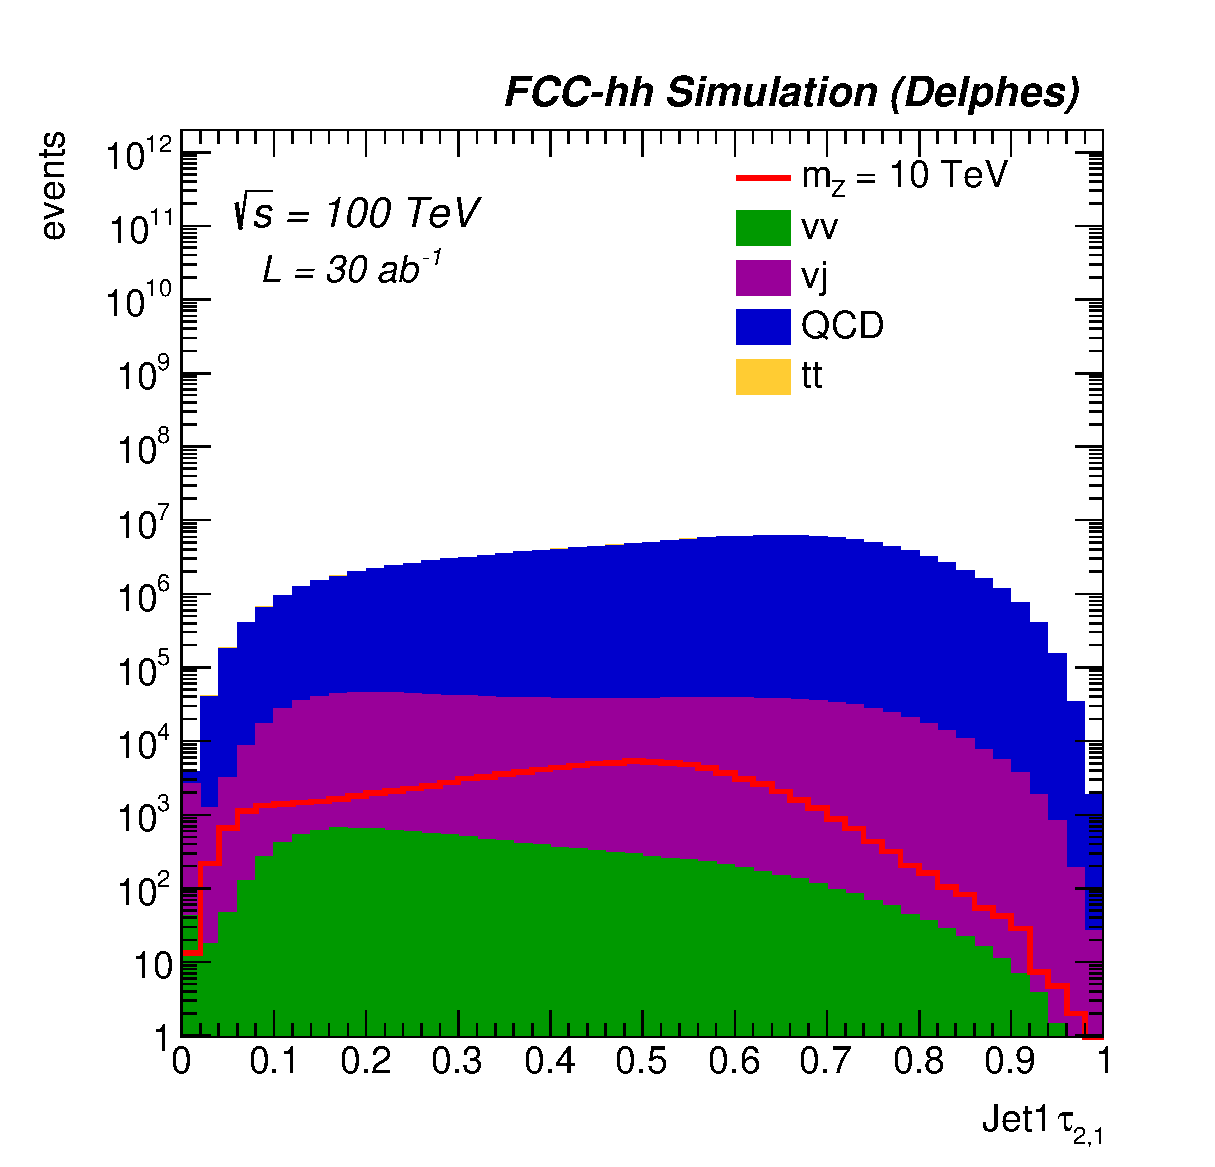
\includegraphics[width=0.32\textwidth]{Fig/Zptt/Jet1_tau21_sel0_nostack_log.eps}
\includegraphics[width=0.32\textwidth]{Fig/Zptt/Jet1_tau32_sel0_nostack_log.eps}
\caption{Variables used for the first step of cuts in cut-based analysis at preselection level for leading jet $\pT$ in \zptt\ analysis : jet mass SD (Soft-Dropped) corrected, jet $\tau_{21}$ and jet $\tau_{32}$. The generated mass of the signal sample is 10 $\TeV$.}
\label{fig:Zptt_sel0_cut}
\end{figure}

\begin{figure}[!htb]\centering
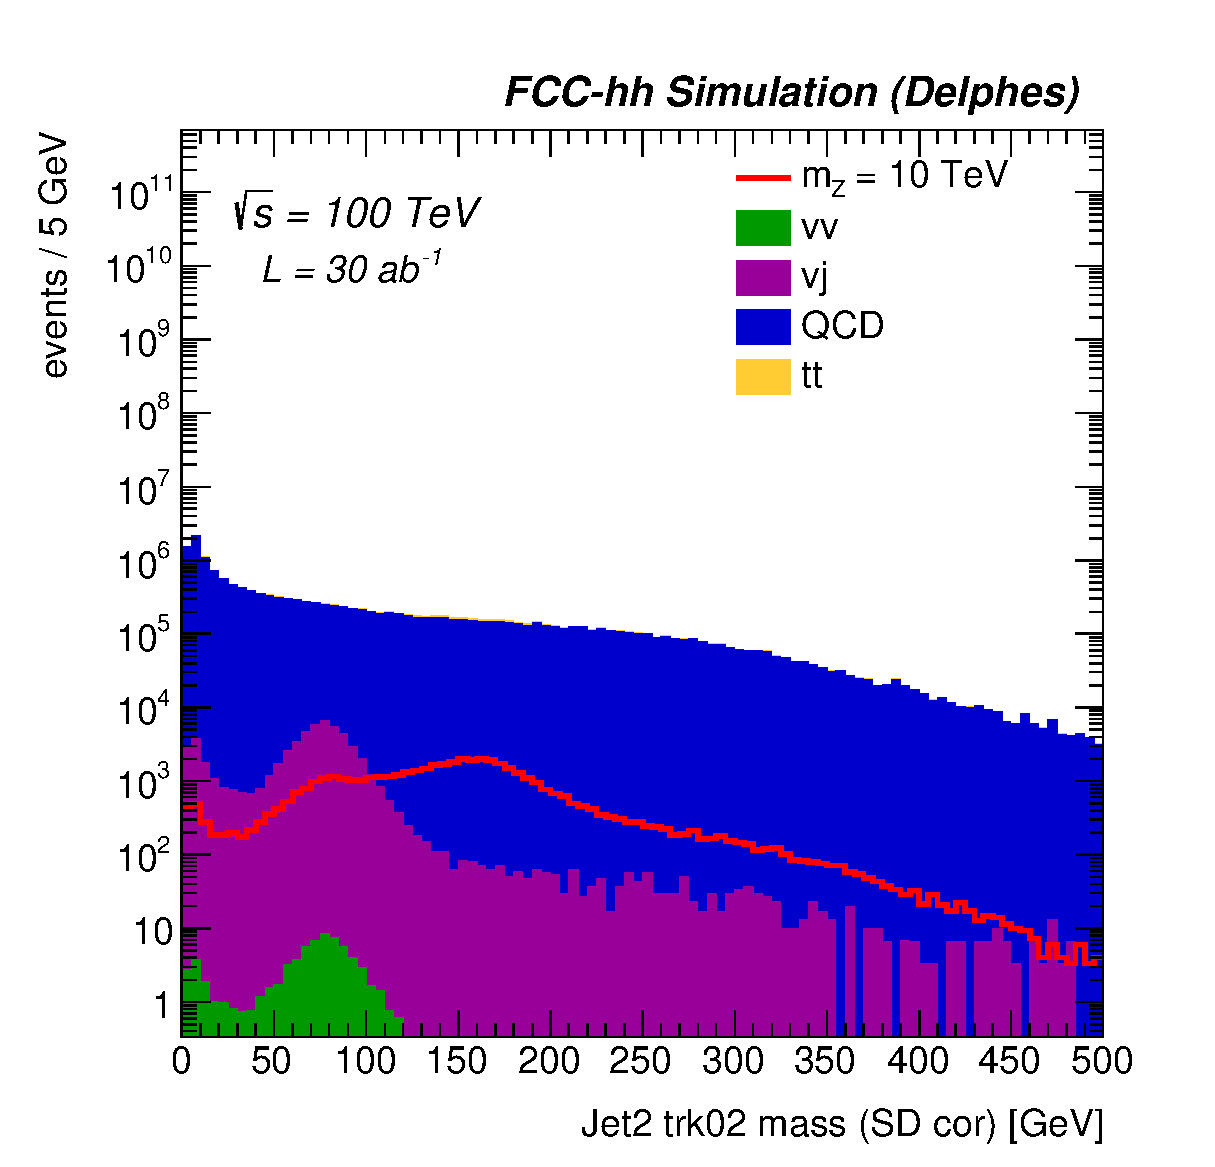
\includegraphics[width=0.32\textwidth]{Fig/Zptt/Jet2_trk02_SD_Cor_m_sel1_nostack_log.eps}
\includegraphics[width=0.32\textwidth]{Fig/Zptt/Jet2_tau21_sel1_nostack_log.eps}
\includegraphics[width=0.32\textwidth]{Fig/Zptt/Jet2_tau32_sel1_nostack_log.eps}
\caption{Variables used for the second step of cuts in cut-based analysis after first set of cuts for second leading jet $\pT$ in \zptt\ analysis : jet mass SD (Soft-Dropped) corrected, jet $\tau_{21}$ and jet $\tau_{32}$. The generated mass of the signal sample is 10 $\TeV$.}
\label{fig:Zptt_sel1_cut}
\end{figure}

\begin{figure}[!htb]\centering
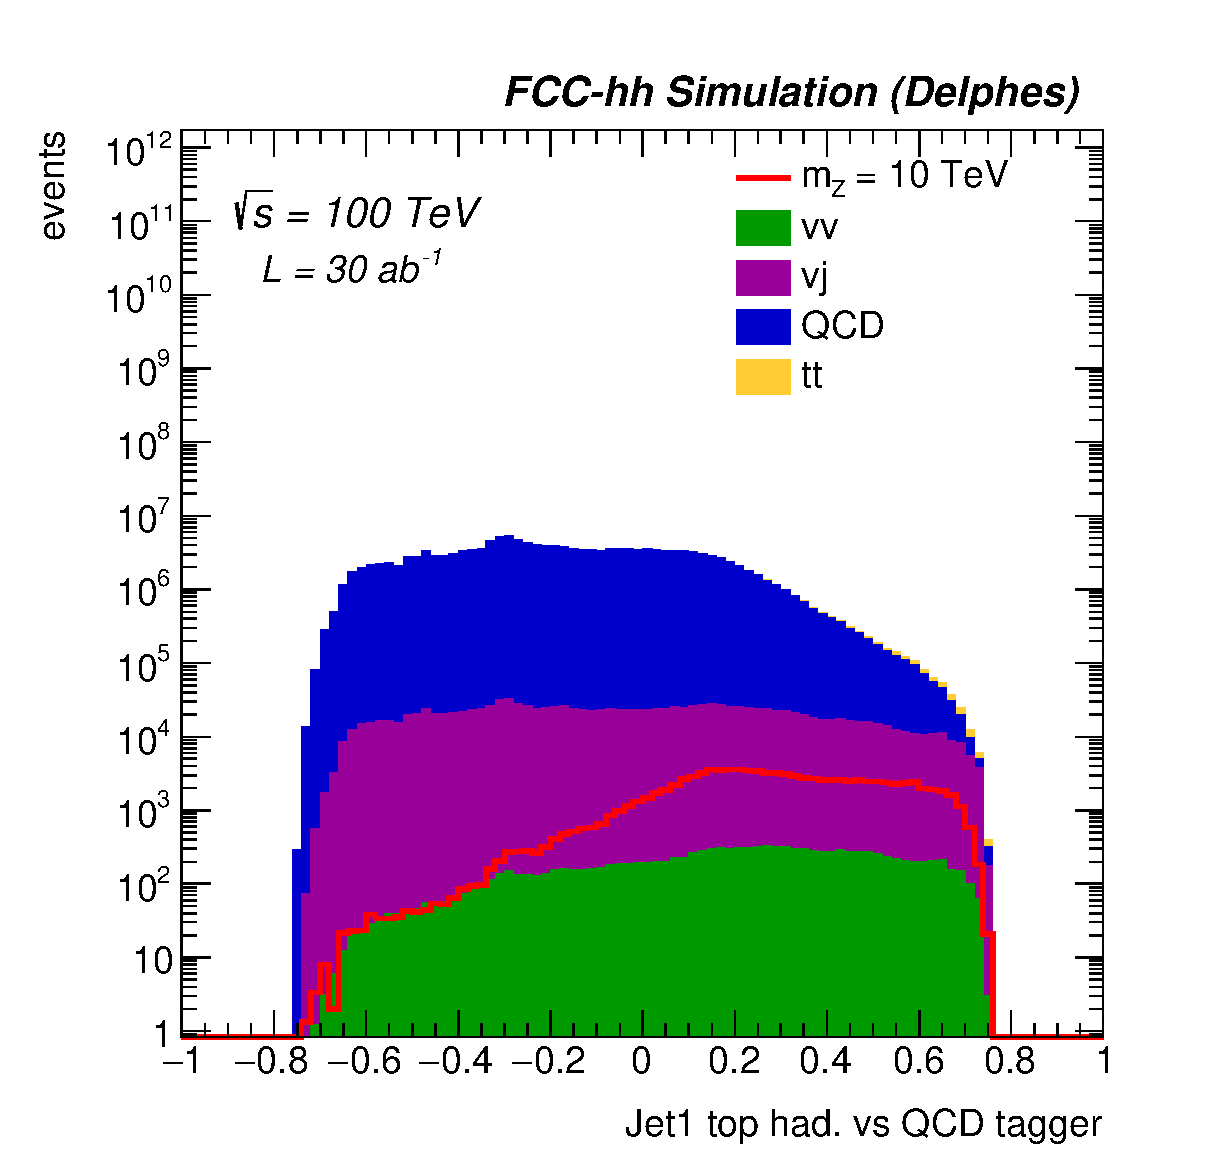
\includegraphics[width=0.32\textwidth]{Fig/Zptt/Jet1_thad_vs_QCD_tagger_sel0_nostack_log.eps}
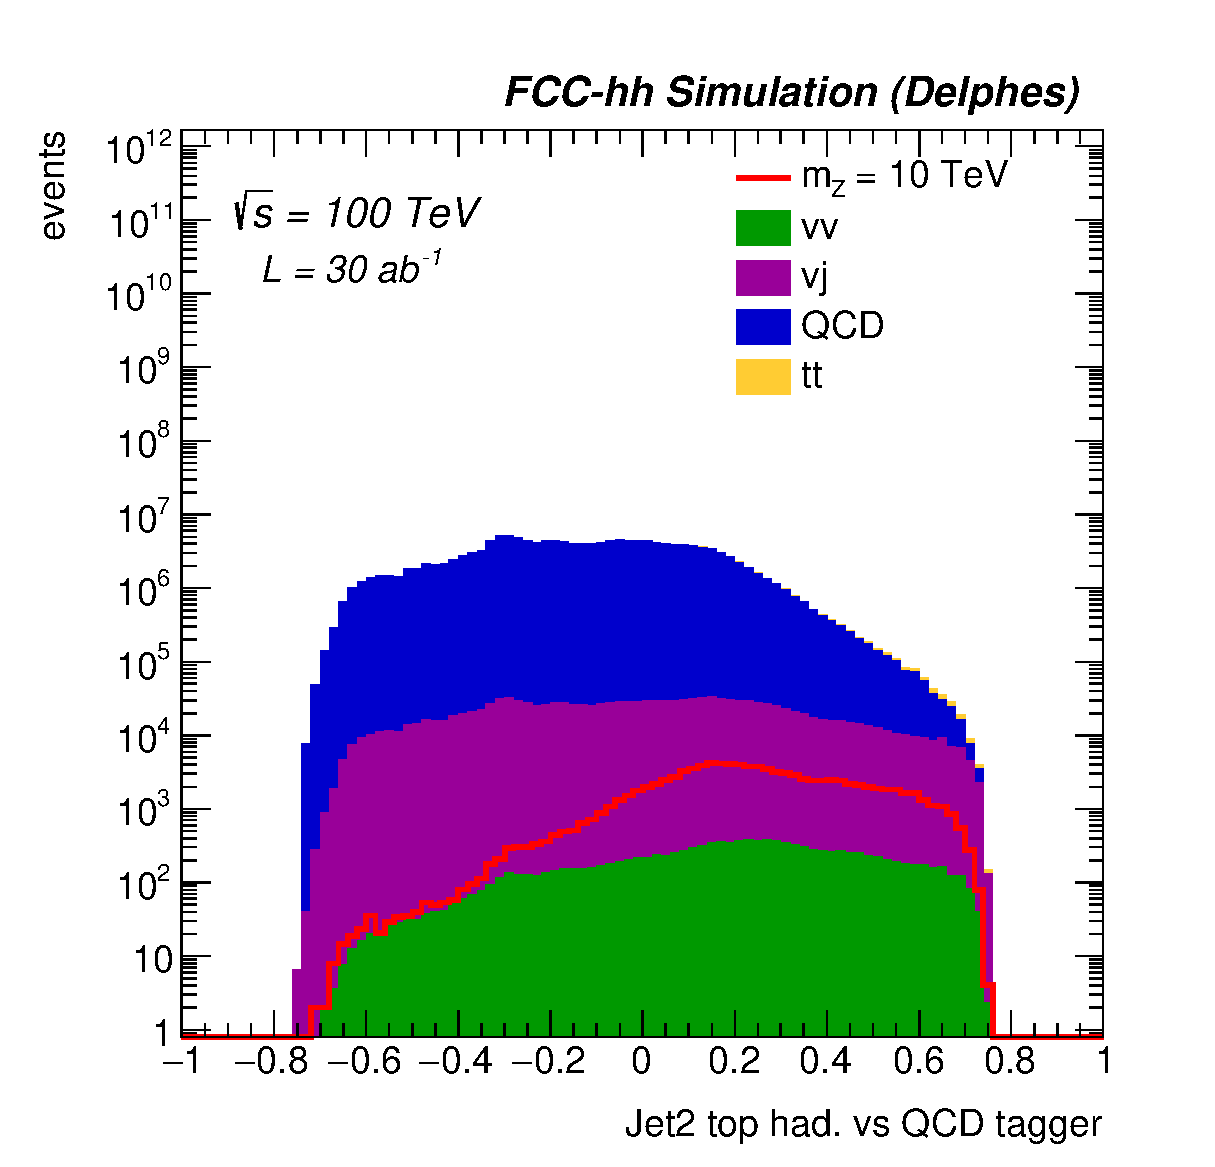
\includegraphics[width=0.32\textwidth]{Fig/Zptt/Jet2_thad_vs_QCD_tagger_sel0_nostack_log.eps}
\caption{top Vs QCD tagger at preselection level for leading jet (left) and second leading jet $\pT$ (right) in \zptt\ analysis. The generated mass of the signal sample is 10 $\TeV$.}
\label{fig:Zptt_sel0_tagger}
\end{figure}

\begin{figure}[!htb]\centering
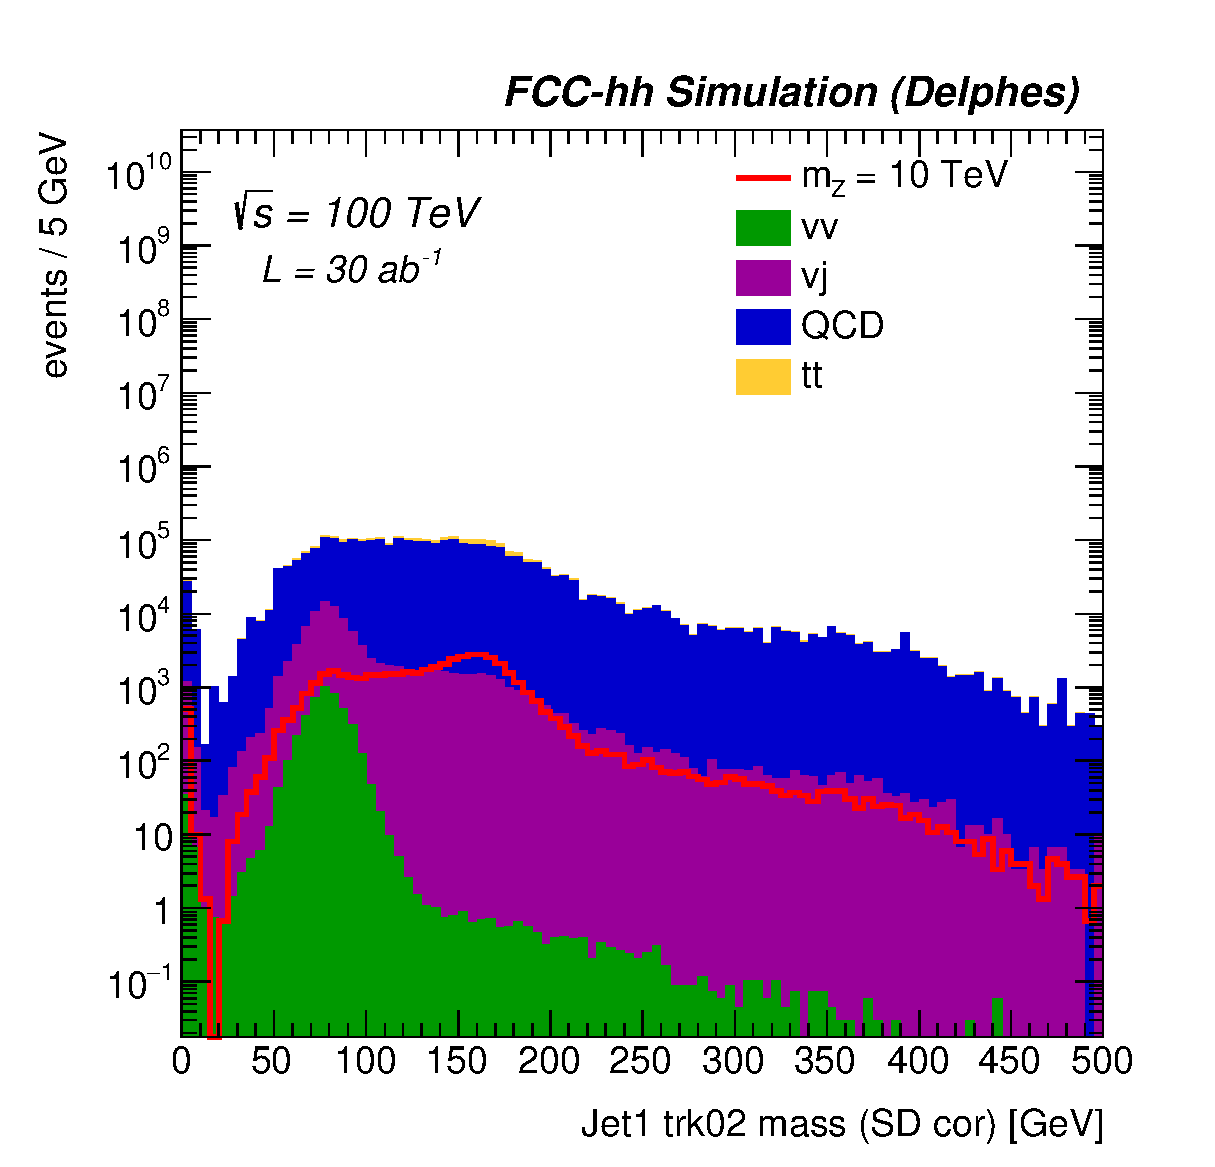
\includegraphics[width=0.32\textwidth]{Fig/Zptt/Jet1_trk02_SD_Cor_m_sel3_nostack_log.eps}
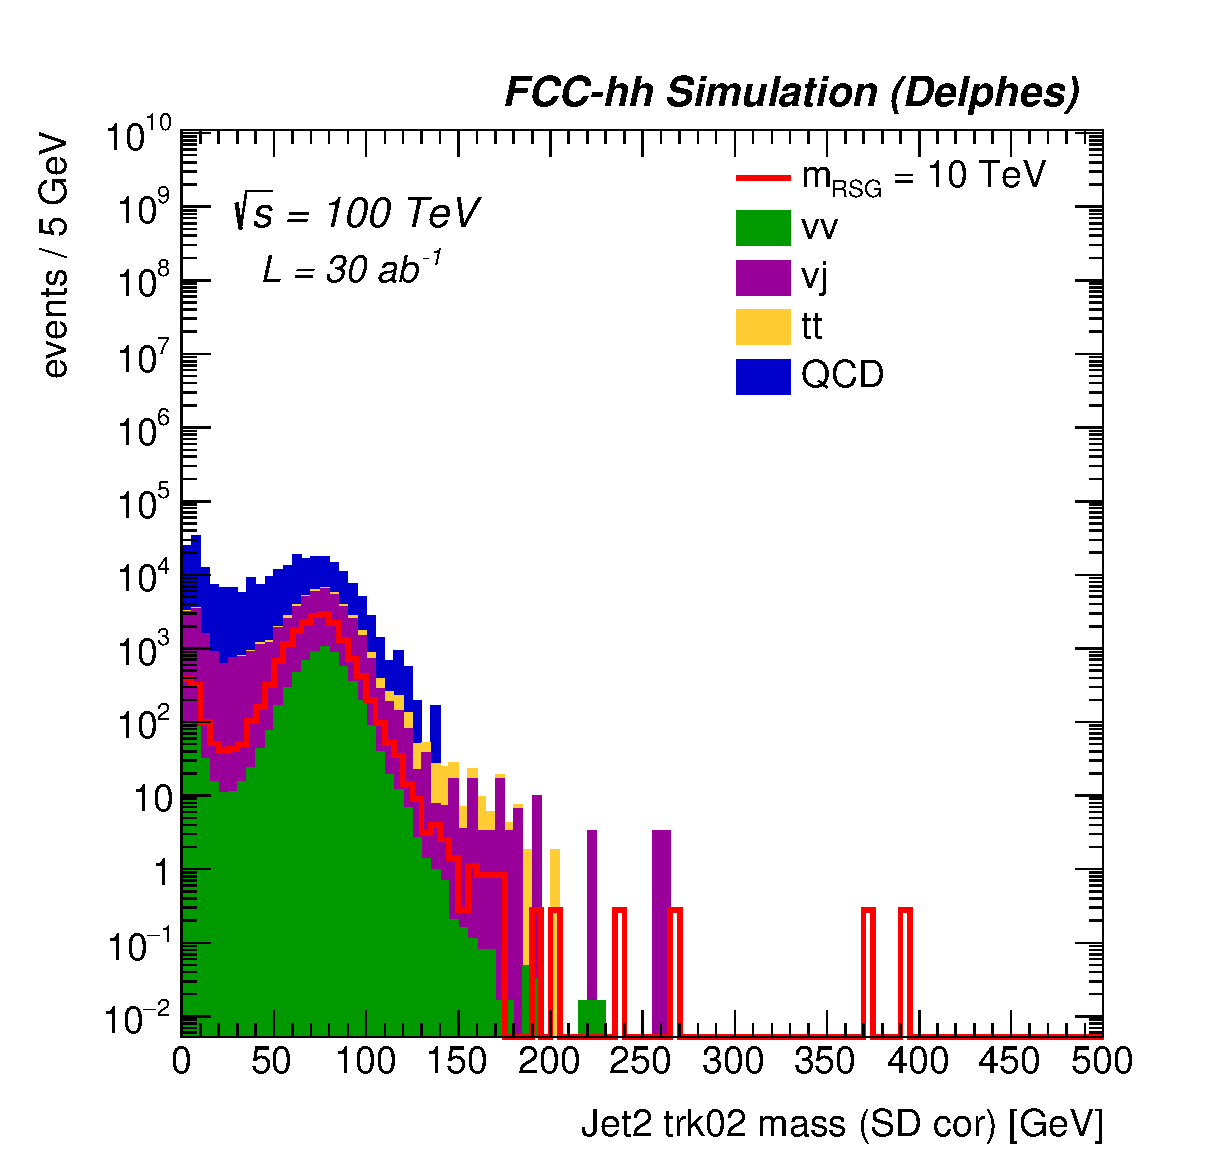
\includegraphics[width=0.32\textwidth]{Fig/Zptt/Jet2_trk02_SD_Cor_m_sel3_nostack_log.eps}
\caption{Jet mass SD (Soft-Dropped) corrected in anti-QCD tagger-based analysis after first set of cuts for leading jet (left) and second leading jet $\pT$ (right) in \zptt\ analysis. The generated mass of the signal sample is 10 $\TeV$.}
\label{fig:Zptt_sel1_tagger}
\end{figure}

% no eps -> useless
%\begin{figure}[!htb]\centering
%\includegraphics[width=0.33\textwidth]{Fig/check_TRF/Zptt/jet12pdgID_QCD5f_redModule_blueDELPHES.png}
%\includegraphics[width=0.33\textwidth]{Fig/check_TRF/Zptt/jet12pdgID_ttbar_redModule_blueDELPHES.png}
%\includegraphics[width=0.33\textwidth]{Fig/check_TRF/Zptt/jet12pdgID_Zptt10TeV_redModule_blueDELPHES.png}
%\includegraphics[width=0.33\textwidth]{Fig/check_TRF/Zptt/TRF2tagex_module_redZptt10TeV_blackQCD_bluettbar.png}
%\caption{Checks of pdgID obtained from recomputation (red) compared to Delphes information (blue) for leading jet (continuous line) and second leading jet $\pT$ (dashed line), and for QCD (top left), $\ttbar$ (top right) and \zptt\ 10 $\TeV$ (bottom left) samples in \zptt\ analysis. Tag Rate Function for a two b-tagged jets event computed from the two leading jets only of the event (bottom right) for QCD (black), $\ttbar$ blue) and \zptt\ 10 $\TeV$ (red) samples.}
%\label{fig:Zptt_TRFchecks}
%\end{figure}

% no eps -> useless
%\begin{figure}[!htb]\centering
%\includegraphics[width=0.33\textwidth]{Fig/check_TRF/tth_boosted/jet12pdgID_ttbb_redModule_blueDELPHES.png}
%\includegraphics[width=0.33\textwidth]{Fig/check_TRF/tth_boosted/jet12pdgID_ttj_redModule_blueDELPHES.png}
%\includegraphics[width=0.33\textwidth]{Fig/check_TRF/tth_boosted/jet12pdgID_ttz_redModule_blueDELPHES.png}
%\includegraphics[width=0.33\textwidth]{Fig/check_TRF/tth_boosted/jet12pdgID_tth_redModule_blueDELPHES.png}
%\caption{Checks of pdgID obtained from recomputation (red) compared to Delphes information (blue) for leading jet (continuous line) and second leading jet $\pT$ (dashed line), and for $\ttbb$ (top left), $\ttj$ (top right), $\ttz$ (bottom left) and $\tthbb$ (bottom right) samples in $\tthbb$ boosted analysis.}
%\label{fig:tthboosted_TRFchecks1}
%\end{figure}

% no eps -> useless
%\begin{figure}[!htb]\centering
%\includegraphics[width=0.33\textwidth]{Fig/check_TRF/tth_boosted/jet34pdgID_ttbb_redModule_blueDELPHES.png}
%\includegraphics[width=0.33\textwidth]{Fig/check_TRF/tth_boosted/jet34pdgID_ttj_redModule_blueDELPHES.png}
%\includegraphics[width=0.33\textwidth]{Fig/check_TRF/tth_boosted/jet34pdgID_ttz_redModule_blueDELPHES.png}
%\includegraphics[width=0.33\textwidth]{Fig/check_TRF/tth_boosted/jet34pdgID_tth_redModule_blueDELPHES.png}
%\caption{Checks of pdgID obtained from recomputation (red) compared to Delphes information (blue) for third leading jet (continuous line) and fourth leading jet $\pT$ (dashed line), and for $\ttbb$ (top left), $\ttj$ (top right), $\ttz$ (bottom left) and $\tthbb$ (bottom right) samples in $\tthbb$ boosted analysis.}
%\label{fig:tthboosted_TRFchecks2}
%\end{figure}

% -> useless
%\begin{figure}[!htb]\centering
%\includegraphics[width=0.495\textwidth]{Fig/Zptt/Mj1j2_pf08_MetCorr_fit_sel2_nostack_log.eps}
%\includegraphics[width=0.495\textwidth]{Fig/Zptt/Mj1j2_pf08_MetCorr_fit_sel4_nostack_log.eps}
%\includegraphics[width=0.495\textwidth]{Fig/Zptt/Mj1j2_pf08_MetCorr_fit_sel5_nostack_log.eps}
%\includegraphics[width=0.495\textwidth]{Fig/Zptt/Mj1j2_pf08_MetCorr_fit_sel6_nostack_log.eps}
%\includegraphics[width=0.495\textwidth]{Fig/Zptt/Mj1j2_pf08_MetCorr_fit_sel7_nostack_log.eps}
%\includegraphics[width=0.495\textwidth]{Fig/Zptt/Mj1j2_pf08_MetCorr_fit_sel8_nostack_log.eps}
%\caption{Zprime mass after the full selection for anaylsis cut-based (left) and anti-QCD tagger based (right), and for the b-tagging scenarios : before b-tag (top), direct 2 b-tag (middle) and Tag Rate Function 2 b-tag (bottom) in \zptt\ analysis. The generated mass of the signal sample is 10 $\TeV$.}
%\label{fig:Zptt_mass_sel_final}
%\end{figure}

%  -> useless
%\begin{figure}[!htb]\centering
%\includegraphics[width=0.495\textwidth]{Fig/Zptt/lim_Zprime_tt_fcc_v02_cut.eps}
%\includegraphics[width=0.495\textwidth]{Fig/Zptt/DiscoveryPotential_tt_cut_rootStyle.eps}
%\includegraphics[width=0.495\textwidth]{Fig/Zptt/lim_Zprime_tt_fcc_v02_tagger.eps}
%\includegraphics[width=0.495\textwidth]{Fig/Zptt/DiscoveryPotential_tt_TC2_tagger_rootStyle.eps}
%\caption{Limit (left) and discovery potential (right) for analysis cut-based with direct b-tagging (top) and anti-QCD tagger-based with direct b-tagging (bottom) in \zptt\ analysis. Default model used for discovery potential is TC2.}
%\label{fig:Zptt_limit_direct}
%\end{figure}

\begin{figure}[!htb]\centering
\includegraphics[width=0.33\textwidth]{Fig/Zptt/lim_Zprime_tt_fcc_v02_cut_TRFbtag.eps}
\includegraphics[width=0.33\textwidth]{Fig/Zptt/DiscoveryPotential_tt_cut_TRFbtag_rootStyle.eps}
\includegraphics[width=0.33\textwidth]{Fig/Zptt/lim_Zprime_tt_fcc_v02_tagger_TRFbtag.eps}
\includegraphics[width=0.33\textwidth]{Fig/Zptt/DiscoveryPotential_tt_SSM_TC2_tagger_TRFbtag_rootStyle.eps}
\caption{Limit (left) and discovery potential (right) for analysis cut-based with TRF b-tagging (top) and anti-QCD tagger-based with TRF b-tagging (bottom) in \zptt\ analysis. Default model used for discovery potential is TC2 in the top plot. The bottom discovery plot shows the comparison between the TC2 default model (red line) and the SSM one (blue line).}
\label{fig:Zptt_limit_trf}
\end{figure}

%\begin{landscape}
\begin{table}[!htb]\centering
\scalebox{0.75}{
\begin{tabular}{|c|c|c|c|c|c|}
\hline
\hline
\multicolumn{2}{|c|}{}          & preselection                                                & cut1                                    & cut2                                    & btag                    \\
\hline
\multicolumn{2}{|c|}{selection} & $Jet_{1,2}^{trk02 SD Corr}~\pT$ > 3 TeV                     & preselection +                          & cut1 +                                  & cut2 +                  \\
\multicolumn{2}{|c|}{}          & |$Jet_{1,2}^{trk02 SD Corr}~\eta$| < 3                      & 0.3 < $Jet_{1}^{trk02}~\tau_{21}$ < 0.7 & 0.3 < $Jet_{2}^{trk02}~\tau_{21}$ < 0.7 & 2 TRF btag              \\
\multicolumn{2}{|c|}{}          & $Jet_{1,2}^{trk02}~\tau_{21,31,32}$ > 0                     & $Jet_{1}^{trk02}~\tau_{32}$ < 0.7       & $Jet_{2}^{trk02}~\tau_{32}$ < 0.75      & (on the 2 leading jets) \\
\multicolumn{2}{|c|}{}          & |$\Delta(Jet_{1}^{trk02}~\eta,Jet_{2}^{trk02}~\eta]$| < 2.4 & $Jet_{1}^{trk02 SD Corr}~M$ > 100 GeV   & $Jet_{2}^{trk02 SD Corr}~M$ > 100 GeV   &                         \\
\multicolumn{2}{|c|}{}          & $M_{Jet_{1},Jet_{2}}^{METcorr}$(pf08) > 5 GeV   &    &   & \\
\hline
\hline
background      & vv            & 41820     & 1470     & 33      & 1     \\
                & vj            & 1610472   & 70864    & 2390    & 5     \\
                & tt            & 1114779   & 472480   & 209660  & 54627 \\
                & QCD           & 154855591 & 16915581 & 2846240 & 10999 \\
                & Total         & 157622662 & 17460395 & 3058323 & 65632 \\
\hline
signal $m_{Z}$= & 10 TeV        & 101529    & 48916    & 27591   & 9278  \\
                & 15 TeV        & 31764     & 14769    & 7460    & 1876  \\
                & 20 TeV        & 7775      & 3561     & 1703    & 304   \\
                & 25 TeV        & 1926      & 867      & 402     & 50    \\
                & 30 TeV        & 485       & 216      & 98      & 9     \\
                & 35 TeV        & 124       & 54       & 25      & 2     \\
\hline
\hline
\end{tabular}}
\caption{Summary of \zptt\ analysis cut-flow for cut-based analysis.}
\label{tab:Zptt_cutflow_cut}
\end{table}
%\end{landscape}

%\begin{landscape}
\begin{table}[!htb]\centering
\scalebox{0.75}{
\begin{tabular}{|c|c|c|c|c|c|}
\hline
\hline
\multicolumn{2}{|c|}{}          & preselection & tagger1 & tagger2 & btag \\
\hline
\multicolumn{2}{|c|}{selection} & $Jet_{1,2}^{trk02 SD Corr}~\pT$ > 3 TeV                     & preselection +                  & tagger1 +                               & tagger2 +               \\
\multicolumn{2}{|c|}{}          & |$Jet_{1,2}^{trk02 SD Corr}~\eta$| < 3                      & $Jet_{1,2}~t/QCD tagger$ > 0.15 & $Jet_{1,2}^{trk02 SD Corr}~M$ > 40 GeV  & 2 TRF btag              \\
\multicolumn{2}{|c|}{}          & $Jet_{1,2}^{trk02}~\tau_{21,31,32}$ > 0                     &                                 &                                         & (on the 2 leading jets) \\
\multicolumn{2}{|c|}{}          & |$\Delta(Jet_{1}^{trk02}~\eta,Jet_{2}^{trk02}~\eta]$| < 2.4 &                                 &                                         &                          \\
\multicolumn{2}{|c|}{}          & $M_{Jet_{1},Jet_{2}}^{METcorr}$(pf08) > 5 GeV   &    &   &   \\
\hline
\hline
background      & vv            & 41820     & 7109    & 6998    & 17    \\
                & vj            & 1610472   & 107224  & 103958  & 264   \\
                & tt            & 1114779   & 257401  & 253907  & 74194 \\
                & QCD           & 154855591 & 2848680 & 2777145 & 11440 \\
                & Total         & 157622662 & 3220414 & 3142008 & 85915 \\
\hline
signal $m_{Z}$= & 10 TeV        & 101529    & 49199   & 48415   & 15602 \\
                & 15 TeV        & 31764     & 13255   & 12943   & 3306  \\
                & 20 TeV        & 7775      & 2594    & 2530    & 501   \\
                & 25 TeV        & 1926      & 491     & 480     & 76    \\
                & 30 TeV        & 485       & 97      & 95      & 13    \\
                & 35 TeV        & 124       & 21      & 21      & 3     \\
\hline
\hline
\end{tabular}}
\caption{Summary of \zptt\ analysis cut-flow for tagger-based analysis.}
\label{tab:Zptt_cutflow_tagger}
\end{table}
%\end{landscape}

\clearpage
\newpage

%%%%%%%%%%%%%%%%%%%%%%%%%%%%%%%%%%%%%%%%%%%%%%%%%%%%%
%%%%%%%%%%%%%%%%%%%%%%%%%%%%%%%%%%%%%%%%%%%%%%%%%%%%%
\section{Appendix : \rsg\ 100 TeV}
\label{appendix:rsg100}

%  -> useless
%\begin{figure}[!htb]\centering
%\includegraphics[width=0.8\textwidth]{Fig/RSGww/rapiditySeparation_sel0_before_cut_nostack_log.eps}
%\caption{Rapidity separation at preselection level before cut on this variable in \rsg\ analysis. The generated mass of the signal sample is 10 $\TeV$.}
%\label{fig:RSGww_sel0_rapidity}
%\end{figure}

\begin{figure}[!htb]\centering
\includegraphics[width=0.33\textwidth]{Fig/RSGww/Jet1_trk02_SD_Cor_m_sel0_nostack_log.eps}
\includegraphics[width=0.33\textwidth]{Fig/RSGww/Jet2_trk02_SD_Cor_m_sel0_nostack_log.eps}
\includegraphics[width=0.33\textwidth]{Fig/RSGww/Jet1_tau21_sel0_nostack_log.eps}
\includegraphics[width=0.33\textwidth]{Fig/RSGww/Jet2_tau21_sel0_nostack_log.eps}
\caption{Variables used for the first step of cuts in cut-based analysis at preselection level for leading jet (left) and second leading jet $\pT$ (right) in \rsg\ analysis : jet mass SD (Soft-Dropped) corrected (top) and jet $\tau_{21}$ (bottom). The generated mass of the signal sample is 10 $\TeV$.}
\label{fig:RSGww_sel0_cut}
\end{figure}

\begin{figure}[!htb]\centering
\includegraphics[width=0.33\textwidth]{Fig/RSGww/Jet1_Flow45_sel1_nostack_log.eps}
\includegraphics[width=0.33\textwidth]{Fig/RSGww/Jet2_Flow45_sel1_nostack_log.eps}
\includegraphics[width=0.33\textwidth]{Fig/RSGww/Jet1_Flow55_sel1_nostack_log.eps}
\includegraphics[width=0.33\textwidth]{Fig/RSGww/Jet2_Flow55_sel1_nostack_log.eps}
\caption{Variables used for the second step of cuts in cut-based analysis after first set of cuts for leading jet (left) and second leading jet $\pT$ (right) in \rsg\ analysis : jet Flow45 (top) and Flow55 (bottom). The generated mass of the signal sample is 10 $\TeV$.}
\label{fig:RSGww_sel1_cut}
\end{figure}

\begin{figure}[!htb]\centering
\includegraphics[width=0.33\textwidth]{Fig/RSGww/Jet1_Whad_vs_QCD_tagger_sel0_nostack_log.eps}
\includegraphics[width=0.33\textwidth]{Fig/RSGww/Jet2_Whad_vs_QCD_tagger_sel0_nostack_log.eps}
\caption{W Vs QCD tagger at preselection level for leading jet (left) and second leading jet $\pT$ (right) in \rsg\ analysis. The generated mass of the signal sample is 10 $\TeV$.}
\label{fig:RSGww_sel0_tagger}
\end{figure}

%  -> ugly
%\begin{figure}[!htb]\centering
%\includegraphics[width=0.33\textwidth]{Fig/RSGww/Jet1_trk02_SD_Cor_m_sel3_nostack_log.eps}
%\includegraphics[width=0.33\textwidth]{Fig/RSGww/Jet2_trk02_SD_Cor_m_sel3_nostack_log.eps}
%\caption{Jet mass SD (Soft-Dropped) corrected in anti-QCD tagger-based analysis after first set of cuts for leading jet (left) and second leading jet $\pT$ (right) in \rsg\ analysis. The generated mass of the signal sample is 10 $\TeV$.}
%\label{fig:RSGww_sel1_tagger}
%\end{figure}

%  -> useless
%\begin{figure}[!htb]\centering
%\includegraphics[width=0.33\textwidth]{Fig/RSGww/Mj1j2_pf08_fit_sel2_nostack_log.eps}
%\includegraphics[width=0.33\textwidth]{Fig/RSGww/Mj1j2_pf08_fit_sel4_nostack_log.eps}
%\caption{RSG mass after the full selection for analysis cut-based (left) and anti-QCD tagger-based (right). The generated mass of the signal sample is 10 $\TeV$.}
%\label{fig:RSGww_mass_sel_final}
%\end{figure}

\begin{figure}[!htb]\centering
\includegraphics[width=0.33\textwidth]{Fig/RSGww/lim_RSGraviton_ww_fcc_v02_cut.eps}
\includegraphics[width=0.33\textwidth]{Fig/RSGww/DiscoveryPotential_ww_cut_rootStyle.eps}
\includegraphics[width=0.33\textwidth]{Fig/RSGww/lim_RSGraviton_ww_fcc_v02_tagger.eps}
\includegraphics[width=0.33\textwidth]{Fig/RSGww/DiscoveryPotential_ww_tagger_rootStyle.eps}
\caption{Limit (left) and discovery potential (right) for analysis cut-based (top) and anti-QCD tagger-based (bottom) in \rsg\ analysis.}
\label{fig:RSWww_limit}
\end{figure}

%\begin{landscape}
\begin{table}[!htb]\centering
\scalebox{0.6}{
\begin{tabular}{|c|c|c|c|c|c|c|}
\hline
\hline
\multicolumn{2}{|c|}{}          & preselection                                                & cut1                                         & cut2                                    & tagger1                         & tagger2                                \\
\hline
\multicolumn{2}{|c|}{selection} & $Jet_{1,2}^{trk02 SD Corr}~\pT$ > 3 TeV                     & preselection +                               & cut1 +                                  & preselection +                  & tagger1 +                              \\
\multicolumn{2}{|c|}{}          & |$Jet_{1,2}^{trk02 SD Corr}~\eta$| < 3                      & 0.3 < $Jet_{1,2}^{trk02}~\tau_{21}$ < 0.6    & $Jet_{1,2}~Flow_{45}$ < 0.07 & $Jet_{1,2}~W/QCD tagger$ > 0.15 & $Jet_{1,2}^{trk02 SD Corr}~M$ > 40 GeV \\
\multicolumn{2}{|c|}{}          & $Jet_{1,2}^{trk02}~\tau_{21,31,32}$ > 0                     & 50 > $Jet_{1,2}^{trk02 SD Corr}~M$ > 100 GeV & $Jet_{1,2}~Flow_{55}$ < 0.07 &                                 &                                        \\
\multicolumn{2}{|c|}{}          & |$\Delta(Jet_{1}^{trk02}~\eta,Jet_{2}^{trk02}~\eta]$| < 2.4 &                                              &                              &                                 &                                        \\
\multicolumn{2}{|c|}{}          & $M_{Jet_{1},Jet_{2}}$(pf08) > 5 GeV &                                              &                              &                                 &                                        \\
\hline
\hline
background      & vv            & 41820     & 10279   & 2952   & 7176   & 6092  \\
                & vj            & 1610472   & 104360  & 26509  & 50485  & 25377 \\
                & tt            & 1114779   & 16446   & 1987   & 3627   & 3185  \\
                & QCD           & 154856149 & 1621365 & 386148 & 225207 & 64484 \\
                & Total         & 157623220 & 1752451 & 417595 & 286495 & 99138 \\
\hline
signal $m_{G}$= & 10 TeV        & 47853     & 20641   & 7036   & 18169  & 15745 \\
                & 15 TeV        & 7242      & 2854    & 1947   & 3744   & 2912  \\
                & 20 TeV        & 1283      & 492     & 412    & 759    & 578   \\
                & 25 TeV        & 259       & 97      & 87     & 159    & 123   \\
                & 30 TeV        & 61        & 23      & 21     & 38     & 30    \\
                & 35 TeV        & 15        & 5       & 5      & 9      & 7     \\
\hline
\hline
\end{tabular}}
\caption{Summary of \rsg\ analysis cut-flow.}
\label{tab:RSGww_cutflow}
\end{table}
%\end{landscape}

\clearpage
\newpage

%%%%%%%%%%%%%%%%%%%%%%%%%%%%%%%%%%%%%%%%%%%%%%%%%%%%%
%%%%%%%%%%%%%%%%%%%%%%%%%%%%%%%%%%%%%%%%%%%%%%%%%%%%%
% NOR SURE IF NEEDED
%\section{Appendix : 27 TeV samples summary}
%\label{appendix:MCtables27}
%
%\begin{table}[!htb]\centering
%\begin{tabular}{|c|c|c|c|}
%\hline
%\hline		
%process & Ngen & generator & k-factor \\
%\hline		
% & & & 2 \\
%\hline
%\hline
%\end{tabular}
%\caption{Summary of generated background samples for HE-LHC analyses. To increase equally the samples statistics in the tails of pT spectrum, the following HT (define HT) binnings has been used : [500, 1000], [1000, 2000], [2000, 5000], [5000, 10000] and [10000, 27000] GeV. 5f stands for 5 flavours jets : u, d, c ,s  and b.}
%\label{tab:MCtable_bkgd27}
%\end{table}
%
%\begin{table}[!htb]\centering
%\begin{tabular}{|c|c|c|c|}
%\hline
%\hline		
%process & Ngen & generator & k-factor \\
%\hline		
% & & & 2 \\
%\hline
%\hline
%\end{tabular}
%\caption{Summary of generated signal samples for HE-LHC analyses.}
%\label{tab:MCtable_sig27}
%\end{table}
%
%%%%%%%%%%%%%%%%%%%%%%%%%%%%%%%%%%%%%%%%%%%%%%%%%%%%%
%%%%%%%%%%%%%%%%%%%%%%%%%%%%%%%%%%%%%%%%%%%%%%%%%%%%%
\section{Appendix : \Zpee\ and \Zpmumu\ 27 TeV}
\label{appendix:zpll27}

\begin{figure}[!htb]
  \centering
  \includegraphics[width=0.33\columnwidth]{Fig/27tev/Zpee_mzp_sel0_nostack_log.eps}
  \includegraphics[width=0.33\columnwidth]{Fig/27tev/Zpmumu_mzp_sel0_nostack_log.eps}
  \includegraphics[width=0.33\columnwidth]{Fig/27tev/lim_Zprime_ll_helhc_v01_allxs.eps}
  \includegraphics[width=0.33\columnwidth]{Fig/27tev/DiscoveryPotential_ll_comb_rootStyle.eps}
  \caption{Invariant mass for a 6~TeV signal after full event selection for \Zpmumu\ (top left) and \Zpmumu\ analysis (top right). Limit versus mass for the di-lepton (ee,$\mu\mu$) channel ( bottom left) and luminosity for a $5\sigma$ discovery ( bottom right) comparing ee,$\mu\mu$ and combined channels.}
  \label{figure:leptonicresonances27:ll}
\end{figure}

\begin{table}[!htb]
   \centering
\begin{tabular}{|l|r|r|}
  \hline
  \hline
 & ee & $\mu\mu$  \\
  \hline
  Drell-Yan    & 162699 &  244802 \\
  \hline
  $\Zp$ 2~TeV  & 737966 & 1040077 \\
  $\Zp$ 4~TeV  &  30351 &   53020 \\
  $\Zp$ 6~TeV  &   2694 &    5343 \\
  $\Zp$ 8~TeV  &    380 &     781 \\
  $\Zp$ 10~TeV &     76 &     151 \\
  $\Zp$ 12~TeV &     23 &      41 \\
  $\Zp$ 14~TeV &     10 &      17 \\
  \hline
  \hline
\end{tabular}
  \caption{Expected number of events for the \Zpee\ and \Zpmumu\ analysis after the full event selection for the various \Zp\ mass hypotheses}
  \label{tab:leptonicresonances27:yieldsll}
\end{table}

\clearpage
\newpage

%%%%%%%%%%%%%%%%%%%%%%%%%%%%%%%%%%%%%%%%%%%%%%%%%%%%%
%%%%%%%%%%%%%%%%%%%%%%%%%%%%%%%%%%%%%%%%%%%%%%%%%%%%%
\section{Appendix : \Zpmumu\ f.a. 27 TeV}
\label{appendix:zpmumufalvano27}

\begin{figure}[!htb]
  \centering
  \includegraphics[width=0.3\columnwidth]{Fig/27tev/mzp_sel0_nostack_log.eps}
  \includegraphics[width=0.3\columnwidth]{Fig/27tev/lim_Zprime_mumu_ano_helhc_v01.eps}
  \includegraphics[width=0.3\columnwidth]{Fig/27tev/DiscoveryPotential_mumu_rootStyle.eps}
  \caption{Left : Invariant mass for a 6~TeV signal after full event selection in \Zpmumu\ f.a. analysis scenario. Limit versus mass (middle) and luminosity for a $5\sigma$ discovery (right).}
  \label{figure:leptonicresonances27:resultsmumu_flav}
\end{figure}

\begin{table}[!htb]
   \centering
\begin{tabular}{|l|r|}
  \hline
  \hline
  Drell-Yan & 47903.9 \\
  \hline
  $\Zp$ 2~TeV  & 751.7 \\
  $\Zp$ 4~TeV  &  94.4 \\
  $\Zp$ 6~TeV  &  14.7 \\
  $\Zp$ 8~TeV  &   3.7 \\
  $\Zp$ 10~TeV &   1.7 \\
  $\Zp$ 12~TeV &   1.2 \\
  $\Zp$ 14~TeV &   1.1 \\
  \hline
  \hline
\end{tabular}
  \caption{Expected number of events for the \Zpmumu\ f.a. analysis after the full event selection for the various \Zp\ mass hypotheses}
  \label{tab:leptonicresonances27:yieldsmumu_flav}
\end{table}

\clearpage
\newpage

%%%%%%%%%%%%%%%%%%%%%%%%%%%%%%%%%%%%%%%%%%%%%%%%%%%%%
%%%%%%%%%%%%%%%%%%%%%%%%%%%%%%%%%%%%%%%%%%%%%%%%%%%%%
\section{Appendix : \Zptata\  27 TeV}
\label{appendix:zptautau27}

\begin{figure}[!htb]
  \centering
  \includegraphics[width=0.32\columnwidth]{Fig/27tev/Zptautau_mt_sel0_nostack_log.eps}
  \includegraphics[width=0.32\columnwidth]{Fig/27tev/lim_Zprime_tautau_helhc_v01.eps}
  \includegraphics[width=0.32\columnwidth]{Fig/27tev/DiscoveryPotential_tautau_rootStyle.eps}
  \caption{Transverse mass (left) for a 6~TeV signal after full event selection for the \Zptata\ analysis. Limit versus mass for the di-tau channel (middle) and luminosity for a $5\sigma$ discovery (right).}
  \label{figure:leptonicresonances27:tautau}
\end{figure}

\begin{table}[!htb]
   \centering
\begin{tabular}{|l|r|r|r|}
  \hline
  \hline
$\Zp$ mass [TeV]  & signal &  Drell-Yan & Di-jet \\
  \hline
  $2$  & 36785 & 4150 & 1259894 \\
  $4$  &  4960 & 4109 & 1323888 \\
  $6$  &   613 & 3896 & 1244660 \\
  $8$  &    94 & 3888 & 1238021 \\
  $10$ &    16 & 4466 & 1551061 \\
  $12$ &     3 & 3948 & 1202671 \\
  $14$ &     1 & 2849 &  645107 \\
  \hline
  \hline
\end{tabular}
  \caption{Expected number of events for the \Zptata\ analysis after the full event selection for the various \Zp\ mass hypotheses}
  \label{tab:leptonicresonances27:yieldstautau}
\end{table}

\clearpage
\newpage

%%%%%%%%%%%%%%%%%%%%%%%%%%%%%%%%%%%%%%%%%%%%%%%%%%%%%
%%%%%%%%%%%%%%%%%%%%%%%%%%%%%%%%%%%%%%%%%%%%%%%%%%%%%
\section{Appendix : \zptt\ 27 TeV}
\label{appendix:zptt27}

\begin{figure}[!htb]
  \centering
  \includegraphics[width=0.30\columnwidth]{Fig/27tev/Zptt_Mj1j2_pf08_MetCorr_fit_sel8_nostack_log.eps}
  \includegraphics[width=0.30\columnwidth]{Fig/27tev/lim_Zprime_tt_helhc_v01.eps}
  \includegraphics[width=0.30\columnwidth]{Fig/27tev/DiscoveryPotential_tt_SSM_TC2_tagger_TRFbtag_rootStyle.eps}
  \caption{Left distribution : invariant mass distribution of the two leading jets for the full selection for a 6~TeV signal for the \zptt\ analysis. Middle distribution : exclusion limit at 95\% CL versus heavy resonance mass. Right distribution : integrated luminosity for a $5\sigma$ discovery as a function of the heavy resonance mass.}
  \label{figure:hadronicresonances27:ttsel08}
\end{figure}

\begin{table}[!htb]\centering
\scalebox{0.9}{
\begin{tabular}{|c|c|c|}
\hline
\hline
signal $m_{Z}$  & 2 TeV  &    84.0 \\
                & 4 TeV  &  4702.8 \\
                & 6 TeV  &  1401.9 \\
                & 8 TeV  &   215.5 \\
                & 10 TeV &    27.6 \\
                & 12 TeV &     3.8 \\
                & 14 TeV &     0.8 \\
\hline
background      & vv     &     5.9 \\
                & vj     &    45.7 \\
                & tt     &   827.4 \\
                & QCD    & 15909.0 \\
                & total  & 16788.0 \\
\hline
\hline
\end{tabular}}
\caption{Final yield of \zptt\ analysis.}
\label{tab:ZpttYield27}
\end{table}

\clearpage
\newpage

%%%%%%%%%%%%%%%%%%%%%%%%%%%%%%%%%%%%%%%%%%%%%%%%%%%%%
%%%%%%%%%%%%%%%%%%%%%%%%%%%%%%%%%%%%%%%%%%%%%%%%%%%%%
\section{Appendix : \rsg\ 27 TeV}
\label{appendix:rsgww27}

\begin{figure}[!htb]
  \centering
  \includegraphics[width=0.30\columnwidth]{Fig/27tev/RSGWW_Mj1j2_pf08_fit_sel4_nostack_log.eps}
  \includegraphics[width=0.30\columnwidth]{Fig/27tev/lim_RSGraviton_ww_helhc_v01.eps}
  \includegraphics[width=0.30\columnwidth]{Fig/27tev/DiscoveryPotential_ww_tagger_rootStyle.eps}
  \caption{Left distribution : invariant mass distribution of the two leading jets for the full selection for a 6~TeV signal for the \rsg\ analysis. Middle distribution : exclusion limit at 95\% CL versus heavy resonance mass. Right distribution : integrated luminosity for a $5\sigma$ discovery as a function of the heavy resonance mass.}
  \label{figure:hadronicresonances27:wwsel04}
\end{figure}

\begin{table}[!htb]\centering
\scalebox{0.9}{
\begin{tabular}{|c|c|c|}
\hline
\hline
signal $m_{RSG}$= & 2 TeV  &  284.6 \\
                  & 4 TeV  &  789.7 \\
                  & 6 TeV  &  245.7 \\
                  & 8 TeV  &   49.0 \\
                  & 10 TeV &    8.7 \\
                  & 12 TeV &    1.4 \\
                  & 14 TeV &    0.8 \\
\hline
background        & vv     &  302.3 \\
                  & vj     &  794.4 \\
                  & tt     &  516.3 \\
                  & QCD    &  547.7 \\
                  & total  & 2160.7 \\
\hline
\hline
\end{tabular}}
\caption{Final yield of \rsg\ analysis.}
\label{tab:RSGwwYield27}
\end{table}

\clearpage
\newpage

%%%%%%%%%%%%%%%%%%%%%%%%%%%%%%%%%%%%%%%%%%%%%%%%%%%%%
%%%%%%%%%%%%%%%%%%%%%%%%%%%%%%%%%%%%%%%%%%%%%%%%%%%%%
\section{Appendix : \qjj\ 27 TeV}
\label{appendix:qstarjj27}

\begin{figure}[!htb]
  \centering
  \includegraphics[width=0.30\columnwidth]{Fig/27tev/qq_Mj1j2_pf04_sel1_nostack_log.eps}
  \includegraphics[width=0.30\columnwidth]{Fig/27tev/lim_Qstar_jj_helhc_v01.eps}
  \includegraphics[width=0.30\columnwidth]{Fig/27tev/DiscoveryPotential_jj_rootStyle.eps}
  \caption{Left distribution : invariant mass distribution of the two leading jets for the full selection for a 6~TeV signal for the \qjj\ analysis. Middle distribution : exclusion limit at 95\% CL versus heavy resonance mass. Right distribution : integrated luminosity for a $5\sigma$ discovery as a function of the heavy resonance mass.}
  \label{figure:hadronicresonances27:qqsel01}
\end{figure}

\begin{table}[!htb]\centering
\scalebox{0.9}{
\begin{tabular}{|c|c|c|}
\hline
\hline
signal $m_{Q^{*}}$  & 2 TeV  &  116820015.2 \\
                    & 4 TeV  &   45971584.5 \\
                    & 6 TeV  &    5064345.4 \\
                    & 8 TeV  &     596530.2 \\
                    & 10 TeV &      76228.5 \\
                    & 12 TeV &       9978.9 \\
                    & 14 TeV &       1314.3 \\
\hline
background          & QCD    & 1144048231.4 \\
\hline
\hline
\end{tabular}}
\caption{Final yield of analysis.}
\label{tab:qqYield27}
\end{table}

\clearpage
\newpage
